\begin{center}
\textbf{\large Supplementary Material: \papertitle}
\end{center}

\section{Autoregressive evolution model} % (fold)
\label{sec:autoregressive_evolution_model}

\begin{itemize}
	\item Show the simplified expression for H=1
	\item discuss irreversibility, with example
\end{itemize}

% section autoregressive_evolution_model (end)

\section{Supplementary figures} % (fold)
\label{sec:supplementary_figures}

\begin{figure}
	\centering
	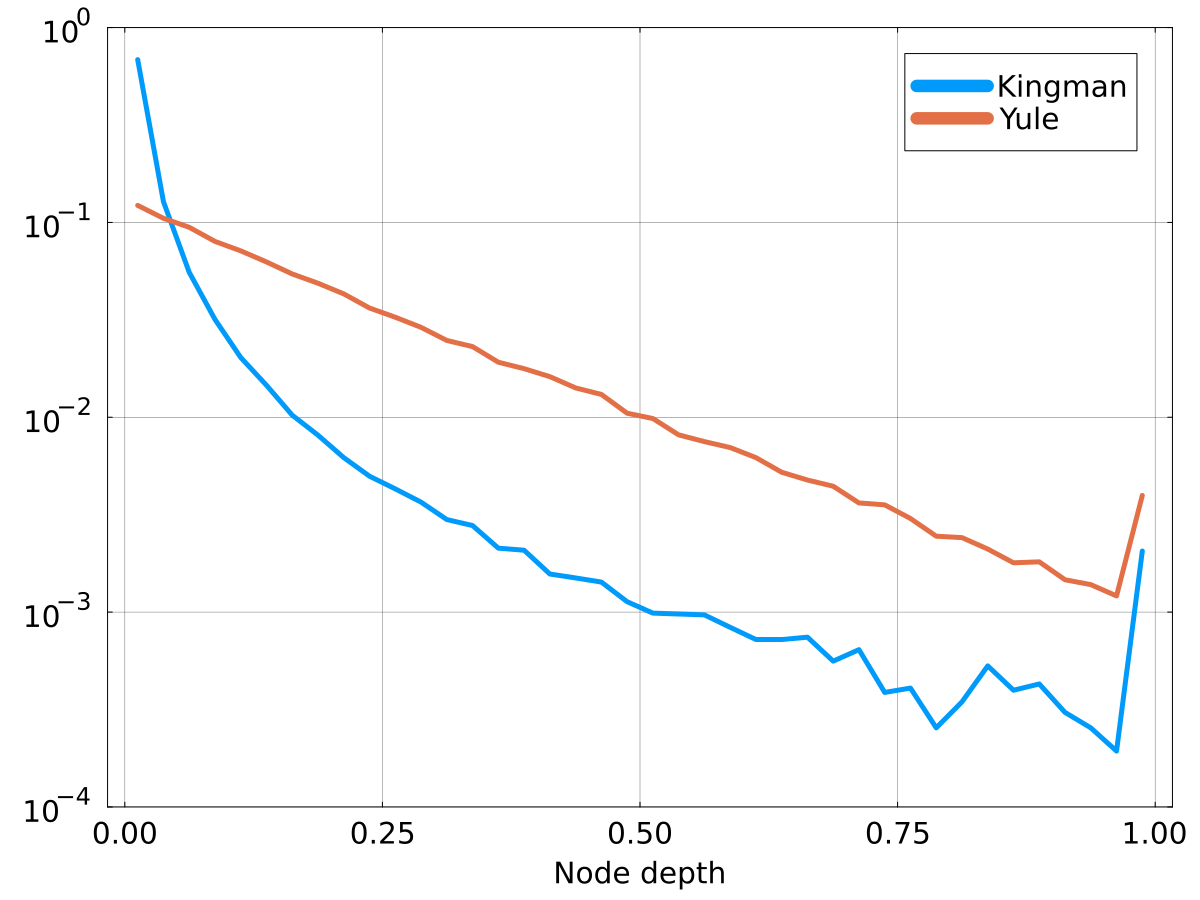
\includegraphics[width=.75\textwidth]{figures/SI/depth_distribution_coalescents.png}
	\caption{
		Distribution of node depth for trees coming from the Kingman and Yule coalescents. 
		Node depth is defined as the distance from a node to the closest leaf. 
		Data is obtained by sampling several trees from each coalescent. 
		Heights of trees are normalized to one. 
		The Kingman process concentrates most of the nodes in close vicinity to the leaves, while the Yule process spreads them more evenly. 
	}
	\label{sfig:depth_distribution_coalescent}
\end{figure}

% section supplementary_figures (end)